\documentclass[12pt]{article}
\usepackage{homework}
\pagestyle{fancy}

% assignment information
\def\course{Classical Mechanics}
\def\assignmentno{Problem Set 5}
\def\assignmentname{Angular Momentum \& Rotational Dynamics}
\def\name{Xin, Wenkang}
\def\time{\today}

\begin{document}

\begin{titlepage}
    \begin{center}
        \large
        \textbf{\course}

        \vfill

        \Huge
        \textbf{\assignmentno}

        \vspace{1.5cm}

        \large{\assignmentname}

        \vfill

        \large
        \name

        \time
    \end{center}
\end{titlepage}


%==========
\pagebreak
\section*{Angular Momentum \& Rotational Dynamics}
%==========


\problem{1}{}
For a uniform disk, its moment of inertia is given by:

\begin{equation}
\begin{split}
    I = \int_{0}^{a} r^{2} m \frac{2\pi r}{\pi a^{2}} \, \mathrm{d}r = \frac{1}{2} m a^{2}
\end{split}
\end{equation}

The angular momentum and kinetic energy of the disk are given by:

\begin{equation}
    L = I \omega = \frac{1}{2} m a^{2} \omega, \quad K = \frac{1}{2} I \omega^{2} = \frac{1}{4} m a^{2} \omega^{2}
\end{equation}

For an inelastic collision, the angular momentum is conserved, so the final angular velocity $\omega'$ is:

\begin{equation}
\begin{split}
    I \omega = 2I \omega' \\
    \omega' = \frac{1}{2} \omega
\end{split}
\end{equation}

and the angular momentum as well as the kinetic energy of the assembly are:

\begin{equation}
    L' = L = \frac{1}{2} m a^{2} \omega, \quad K' = \frac{1}{2} 2I \omega'^{2} = \frac{1}{8} m a^{2} \omega^{2}
\end{equation}
\qed


\problem{2}{}

\subproblem{a}
If the angular deceleration $\alpha = N/I$ is fixed, we have the equation:

\begin{equation}
    N t = I (\omega_{0} - \omega_{1})
\end{equation}

where $I = Mr^{2}/2$ for a cylinder.

This leads to $N = Mr^{2}(\omega_{0} - \omega_{1})/2t$.

\subproblem{b}
If $N = k \omega$ for some positive constant $k$, we have the equation:

\begin{equation}
    I \frac{\mathrm{d}\omega}{\mathrm{d}t} = -k \omega
\end{equation}

Integrating from $\omega_{0}$ to $\omega_{1}$, we have:

\begin{equation}
    \ln{\frac{\omega_{1}}{\omega_{0}}} = -\frac{k}{I} T
\end{equation}

so that $k = I \ln{(\omega_{0}/\omega_{1})}/T$. Then at some $t$, the angular velocity is:

\begin{equation}
    \omega(t) = \omega_{0} e^{-k t/I} = \omega_{0} \left( \frac{\omega_{1}}{\omega_{0}} \right)^{t/T}
\end{equation}

so that the torque is:

\begin{equation}
    N(t) = k \omega(t) = \omega_{0} \frac{Mr^{2}}{2T} \ln{\frac{\omega_{0}}{\omega_{1}}} \left( \frac{\omega_{1}}{\omega_{0}} \right)^{t/T}
\end{equation}

and at $t = T$, the torque evaluates to $N = \omega_{1} Mr^{2}\ln{(\omega_{0}/\omega_{1})}/2T$.
\qed


\problem{3}{}
The reel experiences a tension $T$ and gravity $mg$. For linear motion, we have the equation $ma = mg - T$ and for rotational motion, we have the equation $(mr^{2}/2) \alpha = T r$. For no slipping, $a = \alpha r$. Combining these three equations, we have $T = mg/3$ and :

\begin{equation}
    a = \frac{2g}{3}
\end{equation}
\qed


\problem{4}{}

\subproblem{a}
The angular speed of the cylinder satisfies the equation:

\begin{equation}
    g = \omega^{2} r
\end{equation}

Therefore, the necessary work done, which is just the kinetic energy, is:

\begin{equation}
    W = K = \frac{1}{2} I \omega^{2} = \frac{1}{2} Mgr
\end{equation}

\subproblem{b}
By conservation of angular momentum, the final angular speed is:

\begin{equation}
    \omega' = \frac{I}{I'} \omega = \frac{M}{m + M} \omega
\end{equation}

Thus, the fractional change in kinetic energy is:

\begin{equation}
    \frac{K - K'}{K} = \frac{I\omega^{2} - I'\omega'^{2}}{I\omega^{2}} = \frac{m}{m + M}
\end{equation}

\subproblem{c}
If the astronaut lets go at half-way, he travels perpendicular to the line formed by the spoke at the moment of release in the lab frame. This means that the line joining the point of contact and the centre forms a $\pi/3$ angle with the spoke at the moment of release. The distance to be travelled is $\sqrt{3}r/2$ and the linear speed is $\omega r/2$. The time taken is hence $\sqrt{3}/\omega$. In this time, the spoke travelled an additional angle $\sqrt{3}$. Therefore, the distance from the point of impact to the base of spoke is:

\begin{equation}
    \left( \sqrt{3} - \frac{\pi}{3} \right) r
\end{equation}
\qed


\problem{5}{}
Assuming that the disk is oriented such that the centre axis is in the z-axis. The moment of inertia of the disk is $I = ma^{2}/8$. The couple exerted gives rise to the equation of motion:

\begin{equation}
    I \ddot{\theta} = -c\theta
\end{equation}

which is simple harmonic with the angular frequency $\omega = \sqrt{c/I}$ and period $T = \pi a \sqrt{m/2c}$.

The additional ring causes an increase in the moment of inertia to $I' = 3ma^{2}/8$. The period increases to $T' = \pi a \sqrt{3m/2c}$. If the disk is momentarily at rest at impact, the total energy is all potential energy, which is $c\Theta^{2}/2$ where $\Theta$ is the amplitude of oscillation before impact. If the disk has maximum angular speed, which is $\omega \Theta$, at impact, by conservation of angular momentum:

\begin{equation}
    \omega' = \frac{I}{I'} \omega = \frac{1}{3} \omega
\end{equation}

so that the new total energy is $c\Theta^{2}/6$, which is one third of the original energy.
\qed


\problem{6}{}
By parallel axis theorem, the moment of inertia about $O'$ is $I' = m(a^{2}/2 + x^{2})$. The equation of motion is:

\begin{equation}
    I' \ddot{\theta} = -mgx \sin{\theta} \approx -mgx \theta
\end{equation}

so that the angular frequency is $\omega = \sqrt{mgx/I'}$ and the period is given by:

\begin{equation}
    T = \frac{2\pi}{\omega} = 2\pi \sqrt{\frac{a^{2}/2 + x^{2}}{gx}}
\end{equation}

\begin{center}
    % This file was created with tikzplotlib v0.10.1.
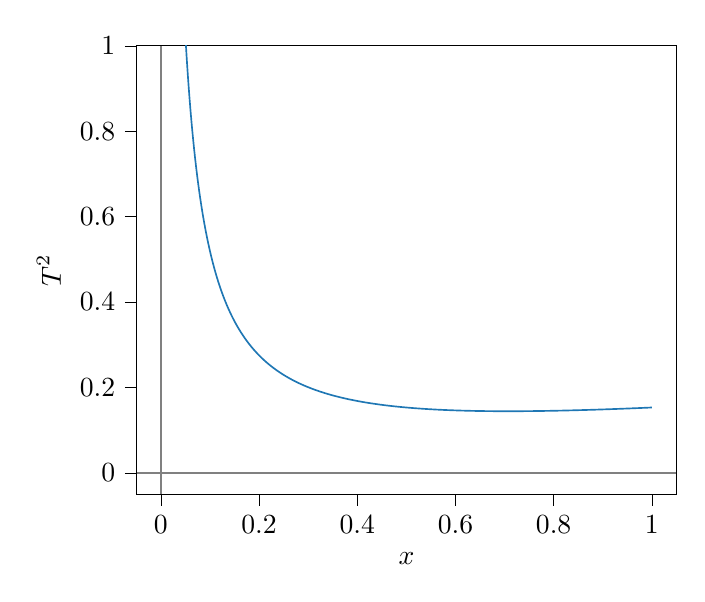
\begin{tikzpicture}

\definecolor{darkgray176}{RGB}{176,176,176}
\definecolor{gray}{RGB}{128,128,128}
\definecolor{steelblue31119180}{RGB}{31,119,180}

\begin{axis}[
tick align=outside,
tick pos=left,
unbounded coords=jump,
x grid style={darkgray176},
xlabel={\(\displaystyle x\)},
xmin=-0.048948948948949, xmax=1.04994994994995,
xtick style={color=black},
y grid style={darkgray176},
ylabel={\(\displaystyle T^{2}\)},
ymin=-0.05, ymax=1,
ytick style={color=black}
]
\addplot [semithick, steelblue31119180]
table {%
0 inf
0.001001001001001 50.9175332314986
0.002002002002002 25.4589196740063
0.003003003003003 16.9727831807343
0.004004004004004 12.7297659535172
0.005005005005005 10.1839964327222
0.00600600600600601 8.48685076513823
0.00700700700700701 7.27463301367481
0.00800800800800801 6.36549520978675
0.00900900900900901 5.65841070428226
0.01001001001001 5.09276350764628
0.011011011011011 4.62997980836921
0.012012012012012 4.24434373211132
0.013013013013013 3.9180519812528
0.014014014014014 3.63838791463664
0.015015015015015 3.39602599541437
0.016016016016016 3.18397207094964
0.017017017017017 2.99687767157936
0.018018018018018 2.83058287645444
0.019019019019019 2.68180353753614
0.02002002002002 2.54791233639348
0.021021021021021 2.42678239620136
0.022022022022022 2.31667354501197
0.023023023023023 2.21614824947715
0.024024024024024 2.12400856514006
0.025025025025025 2.03924821865699
0.026026026026026 1.96101574796784
0.027027027027027 1.88858583353996
0.028028028028028 1.82133677291679
0.029029029029029 1.75873261570474
0.03003003003003 1.70030887156269
0.031031031031031 1.6456609843871
0.032032032032032 1.59443496758736
0.033033033033033 1.5463197420384
0.034034034034034 1.50104082615925
0.035035035035035 1.45835510769252
0.036036036036036 1.41804648685383
0.037037037037037 1.37992222599766
0.038038038038038 1.34380987565171
0.039039039039039 1.30955467346905
0.04004004004004 1.27701733333741
0.041041041041041 1.24607215803357
0.042042042042042 1.21660542149839
0.043043043043043 1.18851397684103
0.044044044044044 1.16170405416073
0.045045045045045 1.13609021865903
0.046046046046046 1.11159446465035
0.047047047047047 1.0881454252309
0.048048048048048 1.06567768073884
0.049049049049049 1.04413115189291
0.05005005005005 1.02345056575434
0.0510510510510511 1.00358498451681
0.0520520520520521 0.984487388666797
0.0530530530530531 0.966114307333317
0.0540540540540541 0.948425489709893
0.0550550550550551 0.931383612321431
0.0560560560560561 0.914954017655343
0.0570570570570571 0.899104480305188
0.0580580580580581 0.883804997306351
0.0590590590590591 0.869027599793508
0.0600600600600601 0.854746183492361
0.0610610610610611 0.840936355884301
0.0620620620620621 0.827575298161599
0.0630630630630631 0.814641640329714
0.0640640640640641 0.802115348018763
0.0650650650650651 0.789977619743165
0.0660660660660661 0.778210793501313
0.0670670670670671 0.766798261739458
0.0680680680680681 0.755724393818775
0.0690690690690691 0.744974465224432
0.0700700700700701 0.734534592842442
0.0710710710710711 0.724391675706086
0.0720720720720721 0.71453334068013
0.0730730730730731 0.704947892609351
0.0740740740740741 0.69562426850908
0.0750750750750751 0.686551995420497
0.0760760760760761 0.67772115159314
0.0770770770770771 0.669122330692157
0.0780780780780781 0.660746608758841
0.0790790790790791 0.652585513680496
0.0800800800800801 0.644630996950059
0.0810810810810811 0.636875407517609
0.0820820820820821 0.629311467555171
0.0830830830830831 0.621932249973467
0.0840840840840841 0.614731157544613
0.0850850850850851 0.607701903498509
0.0860860860860861 0.600838493472967
0.0870870870870871 0.594135208708656
0.0880880880880881 0.587586590389852
0.0890890890890891 0.581187425040865
0.0900900900900901 0.574932730896034
0.0910910910910911 0.568817745168408
0.0920920920920921 0.562837912148731
0.0930930930930931 0.55698887207223
0.0940940940940941 0.551266450696038
0.0950950950950951 0.545666649534883
0.0960960960960961 0.540185636707043
0.0970970970970971 0.534819738346541
0.0980980980980981 0.529565430541111
0.0990990990990991 0.524419331758781
0.1001001001001 0.519378195728858
0.101101101101101 0.514438904745825
0.102102102102102 0.509598463367127
0.103103103103103 0.504853992478073
0.104104104104104 0.500202723699156
0.105105105105105 0.495641994112942
0.106106106106106 0.49116924128945
0.107107107107107 0.486781998590472
0.108108108108108 0.482477890734771
0.109109109109109 0.478254629607396
0.11011011011011 0.474110010297574
0.111111111111111 0.470041907350776
0.112112112112112 0.466048271221564
0.113113113113113 0.462127124914781
0.114114114114114 0.45827656080352
0.115115115115115 0.454494737613117
0.116116116116116 0.450779877561135
0.117117117117117 0.447130263644025
0.118118118118118 0.443544237061748
0.119119119119119 0.440020194772249
0.12012012012012 0.436556587168208
0.121121121121121 0.433151915868995
0.122122122122122 0.429804731621212
0.123123123123123 0.426513632301654
0.124124124124124 0.423277261016895
0.125125125125125 0.4200943042941
0.126126126126126 0.416963490357986
0.127127127127127 0.41388358748918
0.128128128128128 0.410853402459544
0.129129129129129 0.407871779040259
0.13013013013013 0.404937596578779
0.131131131131131 0.402049768640955
0.132132132132132 0.399207241714887
0.133133133133133 0.396408993973241
0.134134134134134 0.393654034090993
0.135135135135135 0.390941400115712
0.136136136136136 0.388270158387686
0.137137137137137 0.385639402507339
0.138138138138138 0.383048252347548
0.139139139139139 0.380495853108589
0.14014014014014 0.377981374413586
0.141141141141141 0.375504009442457
0.142142142142142 0.373062974102442
0.143143143143143 0.370657506233449
0.144144144144144 0.368286864846498
0.145145145145145 0.365950329393684
0.146146146146146 0.363647199068142
0.147147147147147 0.361376792132581
0.148148148148148 0.359138445275041
0.149149149149149 0.356931512990595
0.15015015015015 0.354755366987783
0.151151151151151 0.352609395618624
0.152152152152152 0.350493003331138
0.153153153153153 0.348405610143333
0.154154154154154 0.346346651137681
0.155155155155155 0.344315575975173
0.156156156156156 0.342311848428056
0.157157157157157 0.340334945930432
0.158158158158158 0.338384359145917
0.159159159159159 0.336459591551623
0.16016016016016 0.334560159037733
0.161161161161161 0.332685589522003
0.162162162162162 0.330835422578542
0.163163163163163 0.329009209080252
0.164164164164164 0.327206510854356
0.165165165165165 0.325426900350448
0.166166166166166 0.323669960320538
0.167167167167167 0.321935283510604
0.168168168168168 0.320222472363145
0.169169169169169 0.318531138730308
0.17017017017017 0.316860903597127
0.171171171171171 0.315211396814487
0.172172172172172 0.31358225684139
0.173173173173173 0.311973130496166
0.174174174174174 0.310383672716268
0.175175175175175 0.308813546326288
0.176176176176176 0.3072624218139
0.177177177177177 0.30572997711338
0.178178178178178 0.30421589739644
0.179179179179179 0.302719874870058
0.18018018018018 0.301241608581058
0.181181181181181 0.299780804227164
0.182182182182182 0.298337173974279
0.183183183183183 0.296910436279765
0.184184184184184 0.295500315721474
0.185185185185185 0.294106542832333
0.186186186186186 0.292728853940258
0.187187187187187 0.29136699101321
0.188188188188188 0.290020701509196
0.189189189189189 0.288689738231023
0.19019019019019 0.287373859185652
0.191191191191191 0.28607282744796
0.192192192192192 0.284786411028766
0.193193193193193 0.283514382746952
0.194194194194194 0.282256520105549
0.195195195195195 0.281012605171627
0.196196196196196 0.279782424459867
0.197197197197197 0.278565768819679
0.198198198198198 0.277362433325736
0.199199199199199 0.276172217171812
0.2002002002002 0.274994923567808
0.201201201201201 0.273830359639844
0.202202202202202 0.272678336333326
0.203203203203203 0.271538668318871
0.204204204204204 0.27041117390101
0.205205205205205 0.269295674929548
0.206206206206206 0.268191996713517
0.207207207207207 0.267099967937622
0.208208208208208 0.266019420581092
0.209209209209209 0.264950189838864
0.21021021021021 0.263892114045019
0.211211211211211 0.262845034598396
0.212212212212212 0.261808795890307
0.213213213213213 0.260783245234294
0.214214214214214 0.259768232797852
0.215215215215215 0.258763611536055
0.216216216216216 0.257769237127035
0.217217217217217 0.256784967909232
0.218218218218218 0.255810664820382
0.219219219219219 0.254846191338169
0.22022022022022 0.253891413422504
0.221221221221221 0.252946199459361
0.222222222222222 0.252010420206139
0.223223223223223 0.251083948738488
0.224224224224224 0.250166660398567
0.225225225225225 0.249258432744671
0.226226226226226 0.248359145502209
0.227227227227227 0.247468680515962
0.228228228228228 0.246586921703612
0.229229229229229 0.24571375501048
0.23023023023023 0.244849068365445
0.231231231231231 0.243992751638012
0.232232232232232 0.243144696596488
0.233233233233233 0.242304796867234
0.234234234234234 0.241472947894966
0.235235235235235 0.240649046904062
0.236236236236236 0.239832992860861
0.237237237237237 0.239024686436911
0.238238238238238 0.238224029973146
0.239239239239239 0.23743092744496
0.24024024024024 0.236645284428159
0.241241241241241 0.235867008065755
0.242242242242242 0.235096007035586
0.243243243243243 0.234332191518736
0.244244244244244 0.233575473168729
0.245245245245245 0.232825765081481
0.246246246246246 0.232082981765983
0.247247247247247 0.231347039115696
0.248248248248248 0.230617854380638
0.249249249249249 0.229895346140142
0.25025025025025 0.229179434276274
0.251251251251251 0.22847003994788
0.252252252252252 0.227767085565251
0.253253253253253 0.227070494765393
0.254254254254254 0.226380192387882
0.255255255255255 0.225696104451276
0.256256256256256 0.225018158130097
0.257257257257257 0.224346281732337
0.258258258258258 0.223680404677489
0.259259259259259 0.223020457475096
0.26026026026026 0.222366371703783
0.261261261261261 0.221718079990778
0.262262262262262 0.221075515991904
0.263263263263263 0.220438614372018
0.264264264264264 0.219807310785904
0.265265265265265 0.219181541859595
0.266266266266266 0.218561245172115
0.267267267267267 0.217946359237635
0.268268268268268 0.217336823488025
0.269269269269269 0.216732578255794
0.27027027027027 0.216133564757418
0.271271271271271 0.215539725077022
0.272272272272272 0.214951002150438
0.273273273273273 0.214367339749603
0.274274274274274 0.213788682467299
0.275275275275275 0.213214975702234
0.276276276276276 0.212646165644437
0.277277277277277 0.212082199260979
0.278278278278278 0.211523024281991
0.279279279279279 0.210968589186997
0.28028028028028 0.210418843191524
0.281281281281281 0.209873736234012
0.282282282282282 0.209333218962993
0.283283283283283 0.208797242724547
0.284284284284284 0.20826575955002
0.285285285285285 0.207738722144001
0.286286286286286 0.207216083872557
0.287287287287287 0.206697798751701
0.288288288288288 0.206183821436115
0.289289289289289 0.205674107208097
0.29029029029029 0.205168611966742
0.291291291291291 0.204667292217341
0.292292292292292 0.204170105061005
0.293293293293293 0.203677008184493
0.294294294294294 0.203187959850258
0.295295295295295 0.202702918886682
0.296296296296296 0.202221844678522
0.297297297297297 0.201744697157541
0.298298298298298 0.201271436793333
0.299299299299299 0.200802024584323
0.3003003003003 0.20033642204896
0.301301301301301 0.199874591217075
0.302302302302302 0.199416494621415
0.303303303303303 0.198962095289343
0.304304304304304 0.198511356734706
0.305305305305305 0.198064242949857
0.306306306306306 0.197620718397837
0.307307307307307 0.197180748004709
0.308308308308308 0.196744297152044
0.309309309309309 0.196311331669546
0.31031031031031 0.195881817827824
0.311311311311311 0.19545572233131
0.312312312312312 0.1950330123113
0.313313313313313 0.194613655319136
0.314314314314314 0.194197619319521
0.315315315315315 0.193784872683955
0.316316316316316 0.193375384184298
0.317317317317317 0.192969122986455
0.318318318318318 0.192566058644185
0.319319319319319 0.192166161093013
0.32032032032032 0.191769400644273
0.321321321321321 0.191375747979252
0.322322322322322 0.190985174143442
0.323323323323323 0.190597650540907
0.324324324324324 0.190213148928745
0.325325325325325 0.189831641411662
0.326326326326326 0.189453100436634
0.327327327327327 0.18907749878768
0.328328328328328 0.18870480958072
0.329329329329329 0.188335006258532
0.33033033033033 0.1879680625858
0.331331331331331 0.18760395264425
0.332332332332332 0.187242650827879
0.333333333333333 0.18688413183826
0.334334334334334 0.186528370679945
0.335335335335335 0.186175342655937
0.336336336336336 0.18582502336325
0.337337337337337 0.185477388688549
0.338338338338338 0.185132414803865
0.339339339339339 0.184790078162382
0.34034034034034 0.184450355494308
0.341341341341341 0.18411322380281
0.342342342342342 0.183778660360022
0.343343343343343 0.183446642703128
0.344344344344344 0.183117148630507
0.345345345345345 0.182790156197948
0.346346346346346 0.182465643714929
0.347347347347347 0.182143589740966
0.348348348348348 0.181823973082014
0.349349349349349 0.181506772786941
0.35035035035035 0.181191968144058
0.351351351351351 0.180879538677704
0.352352352352352 0.180569464144897
0.353353353353353 0.180261724532039
0.354354354354354 0.179956300051671
0.355355355355355 0.179653171139295
0.356356356356356 0.179352318450235
0.357357357357357 0.179053722856565
0.358358358358358 0.178757365444078
0.359359359359359 0.178463227509309
0.36036036036036 0.178171290556612
0.361361361361361 0.177881536295275
0.362362362362362 0.177593946636698
0.363363363363363 0.177308503691601
0.364364364364364 0.17702518976729
0.365365365365365 0.176743987364964
0.366366366366366 0.176464879177066
0.367367367367367 0.176187848084678
0.368368368368368 0.175912877154955
0.369369369369369 0.175639949638607
0.37037037037037 0.175369048967418
0.371371371371371 0.175100158751804
0.372372372372372 0.174833262778414
0.373373373373373 0.174568345007766
0.374374374374374 0.174305389571924
0.375375375375375 0.17404438077221
0.376376376376376 0.173785303076951
0.377377377377377 0.173528141119269
0.378378378378378 0.173272879694898
0.379379379379379 0.173019503760038
0.38038038038038 0.172767998429246
0.381381381381381 0.172518348973356
0.382382382382382 0.172270540817434
0.383383383383383 0.172024559538765
0.384384384384384 0.171780390864871
0.385385385385385 0.171538020671558
0.386386386386386 0.171297434980998
0.387387387387387 0.171058619959836
0.388388388388388 0.17082156191733
0.389389389389389 0.170586247303515
0.39039039039039 0.170352662707403
0.391391391391391 0.170120794855199
0.392392392392392 0.169890630608557
0.393393393393393 0.169662156962855
0.394394394394394 0.169435361045497
0.395395395395395 0.169210230114242
0.396396396396396 0.168986751555559
0.397397397397397 0.168764912883006
0.398398398398398 0.168544701735631
0.399399399399399 0.168326105876404
0.4004004004004 0.168109113190663
0.401401401401401 0.167893711684591
0.402402402402402 0.167679889483714
0.403403403403403 0.167467634831418
0.404404404404404 0.167256936087489
0.405405405405405 0.167047781726681
0.406406406406406 0.166840160337296
0.407407407407407 0.166634060619789
0.408408408408408 0.166429471385399
0.409409409409409 0.166226381554785
0.41041041041041 0.166024780156701
0.411411411411411 0.165824656326676
0.412412412412412 0.16562599930572
0.413413413413413 0.165428798439044
0.414414414414414 0.165233043174806
0.415415415415415 0.165038723062869
0.416416416416416 0.164845827753575
0.417417417417417 0.164654346996547
0.418418418418418 0.164464270639495
0.419419419419419 0.164275588627049
0.42042042042042 0.164088290999606
0.421421421421421 0.163902367892189
0.422422422422422 0.163717809533328
0.423423423423423 0.163534606243956
0.424424424424424 0.163352748436317
0.425425425425425 0.163172226612893
0.426426426426426 0.162993031365345
0.427427427427427 0.162815153373466
0.428428428428428 0.162638583404157
0.429429429429429 0.162463312310407
0.43043043043043 0.162289331030293
0.431431431431431 0.162116630585994
0.432432432432432 0.161945202082817
0.433433433433433 0.161775036708236
0.434434434434434 0.161606125730949
0.435435435435435 0.161438460499939
0.436436436436436 0.161272032443557
0.437437437437437 0.161106833068615
0.438438438438438 0.160942853959485
0.439439439439439 0.160780086777221
0.44044044044044 0.160618523258686
0.441441441441441 0.160458155215691
0.442442442442442 0.160298974534149
0.443443443443443 0.160140973173236
0.444444444444444 0.159984143164571
0.445445445445445 0.159828476611397
0.446446446446446 0.15967396568778
0.447447447447447 0.159520602637816
0.448448448448448 0.159368379774853
0.449449449449449 0.159217289480713
0.45045045045045 0.159067324204939
0.451451451451451 0.158918476464037
0.452452452452452 0.158770738840741
0.453453453453453 0.158624103983279
0.454454454454454 0.158478564604652
0.455455455455455 0.158334113481922
0.456456456456456 0.158190743455511
0.457457457457457 0.158048447428507
0.458458458458458 0.157907218365978
0.459459459459459 0.157767049294302
0.46046046046046 0.157627933300495
0.461461461461461 0.157489863531554
0.462462462462462 0.157352833193812
0.463463463463463 0.157216835552293
0.464464464464464 0.157081863930084
0.465465465465465 0.156947911707703
0.466466466466466 0.156814972322491
0.467467467467467 0.156683039267999
0.468468468468468 0.156552106093391
0.469469469469469 0.156422166402844
0.47047047047047 0.156293213854972
0.471471471471471 0.156165242162242
0.472472472472472 0.156038245090406
0.473473473473473 0.155912216457934
0.474474474474474 0.155787150135464
0.475475475475475 0.155663040045249
0.476476476476476 0.155539880160615
0.477477477477477 0.155417664505426
0.478478478478478 0.155296387153556
0.479479479479479 0.155176042228366
0.48048048048048 0.15505662390219
0.481481481481481 0.154938126395823
0.482482482482482 0.154820543978022
0.483483483483483 0.154703870965006
0.484484484484485 0.154588101719971
0.485485485485485 0.154473230652597
0.486486486486486 0.154359252218579
0.487487487487487 0.154246160919149
0.488488488488488 0.15413395130061
0.48948948948949 0.154022617953876
0.49049049049049 0.153912155514019
0.491491491491491 0.153802558659816
0.492492492492492 0.153693822113304
0.493493493493493 0.153585940639347
0.494494494494495 0.153478909045195
0.495495495495495 0.153372722180062
0.496496496496497 0.153267374934699
0.497497497497497 0.15316286224098
0.498498498498498 0.153059179071485
0.4994994994995 0.152956320439094
0.500500500500501 0.152854281396585
0.501501501501502 0.152753057036234
0.502502502502503 0.152652642489422
0.503503503503503 0.152553032926247
0.504504504504504 0.152454223555141
0.505505505505506 0.152356209622487
0.506506506506507 0.152258986412246
0.507507507507508 0.152162549245589
0.508508508508508 0.152066893480524
0.509509509509509 0.151972014511543
0.510510510510511 0.151877907769255
0.511511511511512 0.151784568720041
0.512512512512513 0.1516919928657
0.513513513513513 0.151600175743102
0.514514514514514 0.151509112923853
0.515515515515516 0.151418800013953
0.516516516516517 0.151329232653463
0.517517517517518 0.151240406516178
0.518518518518518 0.1511523173093
0.519519519519519 0.151064960773115
0.520520520520521 0.150978332680677
0.521521521521522 0.150892428837493
0.522522522522523 0.150807245081209
0.523523523523523 0.150722777281309
0.524524524524524 0.150639021338806
0.525525525525526 0.150555973185943
0.526526526526527 0.150473628785896
0.527527527527528 0.150391984132484
0.528528528528528 0.150311035249873
0.529529529529529 0.150230778192293
0.530530530530531 0.150151209043752
0.531531531531532 0.15007232391776
0.532532532532533 0.149994118957046
0.533533533533533 0.149916590333288
0.534534534534534 0.14983973424684
0.535535535535536 0.149763546926465
0.536536536536537 0.149688024629069
0.537537537537538 0.149613163639439
0.538538538538539 0.149538960269987
0.539539539539539 0.149465410860489
0.540540540540541 0.149392511777833
0.541541541541542 0.149320259415771
0.542542542542543 0.149248650194669
0.543543543543544 0.149177680561261
0.544544544544544 0.149107346988411
0.545545545545546 0.149037645974866
0.546546546546547 0.148968574045027
0.547547547547548 0.148900127748708
0.548548548548549 0.148832303660908
0.54954954954955 0.148765098381582
0.550550550550551 0.14869850853541
0.551551551551552 0.148632530771576
0.552552552552553 0.148567161763545
0.553553553553554 0.148502398208846
0.554554554554555 0.14843823682885
0.555555555555556 0.148374674368558
0.556556556556557 0.14831170759639
0.557557557557558 0.148249333303971
0.558558558558559 0.148187548305927
0.55955955955956 0.148126349439675
0.560560560560561 0.148065733565224
0.561561561561562 0.148005697564971
0.562562562562563 0.147946238343502
0.563563563563564 0.147887352827395
0.564564564564565 0.147829037965026
0.565565565565566 0.147771290726375
0.566566566566567 0.147714108102837
0.567567567567568 0.147657487107028
0.568568568568569 0.147601424772607
0.56956956956957 0.147545918154081
0.570570570570571 0.147490964326631
0.571571571571572 0.147436560385926
0.572572572572573 0.147382703447943
0.573573573573574 0.147329390648794
0.574574574574575 0.147276619144549
0.575575575575576 0.147224386111059
0.576576576576577 0.14717268874379
0.577577577577578 0.147121524257648
0.578578578578579 0.147070889886815
0.57957957957958 0.147020782884578
0.580580580580581 0.146971200523171
0.581581581581582 0.146922140093603
0.582582582582583 0.146873598905504
0.583583583583584 0.146825574286963
0.584584584584585 0.14677806358437
0.585585585585586 0.146731064162257
0.586586586586587 0.146684573403148
0.587587587587588 0.146638588707402
0.588588588588589 0.146593107493064
0.58958958958959 0.146548127195711
0.590590590590591 0.146503645268309
0.591591591591592 0.146459659181061
0.592592592592593 0.146416166421263
0.593593593593594 0.146373164493161
0.594594594594595 0.146330650917807
0.595595595595596 0.146288623232918
0.596596596596597 0.146247078992736
0.597597597597598 0.146206015767892
0.598598598598599 0.146165431145265
0.5995995995996 0.146125322727849
0.600600600600601 0.146085688134618
0.601601601601602 0.146046525000392
0.602602602602603 0.146007830975709
0.603603603603604 0.14596960372669
0.604604604604605 0.145931840934913
0.605605605605606 0.145894540297283
0.606606606606607 0.14585769952591
0.607607607607608 0.145821316347979
0.608608608608609 0.145785388505626
0.60960960960961 0.145749913755819
0.610610610610611 0.145714889870235
0.611611611611612 0.145680314635137
0.612612612612613 0.145646185851259
0.613613613613614 0.145612501333683
0.614614614614615 0.145579258911729
0.615615615615616 0.145546456428831
0.616616616616617 0.14551409174243
0.617617617617618 0.145482162723855
0.618618618618619 0.145450667258215
0.61961961961962 0.145419603244282
0.620620620620621 0.145388968594388
0.621621621621622 0.14535876123431
0.622622622622623 0.145328979103165
0.623623623623624 0.145299620153301
0.624624624624625 0.145270682350193
0.625625625625626 0.145242163672337
0.626626626626627 0.145214062111145
0.627627627627628 0.145186375670844
0.628628628628629 0.145159102368371
0.62962962962963 0.145132240233278
0.630630630630631 0.145105787307622
0.631631631631632 0.145079741645877
0.632632632632633 0.145054101314827
0.633633633633634 0.145028864393474
0.634634634634635 0.14500402897294
0.635635635635636 0.144979593156369
0.636636636636637 0.144955555058838
0.637637637637638 0.144931912807259
0.638638638638639 0.144908664540286
0.63963963963964 0.144885808408227
0.640640640640641 0.14486334257295
0.641641641641642 0.144841265207792
0.642642642642643 0.144819574497473
0.643643643643644 0.144798268638004
0.644644644644645 0.144777345836602
0.645645645645646 0.144756804311601
0.646646646646647 0.144736642292368
0.647647647647648 0.144716858019216
0.648648648648649 0.144697449743321
0.64964964964965 0.144678415726637
0.650650650650651 0.144659754241813
0.651651651651652 0.144641463572114
0.652652652652653 0.144623542011333
0.653653653653654 0.144605987863719
0.654654654654655 0.14458879944389
0.655655655655656 0.144571975076757
0.656656656656657 0.144555513097444
0.657657657657658 0.144539411851213
0.658658658658659 0.144523669693384
0.65965965965966 0.14450828498926
0.660660660660661 0.144493256114051
0.661661661661662 0.144478581452801
0.662662662662663 0.14446425940031
0.663663663663664 0.144450288361064
0.664664664664665 0.144436666749158
0.665665665665666 0.14442339298823
0.666666666666667 0.144410465511383
0.667667667667668 0.144397882761117
0.668668668668669 0.144385643189259
0.66966966966967 0.144373745256893
0.670670670670671 0.144362187434289
0.671671671671672 0.144350968200837
0.672672672672673 0.144340086044979
0.673673673673674 0.14432953946414
0.674674674674675 0.144319326964663
0.675675675675676 0.144309447061741
0.676676676676677 0.144299898279354
0.677677677677678 0.144290679150204
0.678678678678679 0.144281788215647
0.67967967967968 0.144273224025633
0.680680680680681 0.144264985138643
0.681681681681682 0.144257070121624
0.682682682682683 0.144249477549928
0.683683683683684 0.14424220600725
0.684684684684685 0.144235254085568
0.685685685685686 0.144228620385082
0.686686686686687 0.144222303514155
0.687687687687688 0.144216302089251
0.688688688688689 0.144210614734878
0.68968968968969 0.144205240083531
0.690690690690691 0.144200176775632
0.691691691691692 0.144195423459472
0.692692692692693 0.144190978791157
0.693693693693694 0.144186841434548
0.694694694694695 0.144183010061209
0.695695695695696 0.144179483350348
0.696696696696697 0.144176259988767
0.697697697697698 0.144173338670799
0.698698698698699 0.144170718098264
0.6996996996997 0.144168396980409
0.700700700700701 0.144166374033856
0.701701701701702 0.144164647982552
0.702702702702703 0.144163217557713
0.703703703703704 0.144162081497775
0.704704704704705 0.144161238548344
0.705705705705706 0.144160687462138
0.706706706706707 0.144160426998948
0.707707707707708 0.144160455925577
0.708708708708709 0.144160773015798
0.70970970970971 0.1441613770503
0.710710710710711 0.144162266816644
0.711711711711712 0.144163441109208
0.712712712712713 0.144164898729148
0.713713713713714 0.144166638484341
0.714714714714715 0.144168659189346
0.715715715715716 0.144170959665353
0.716716716716717 0.144173538740136
0.717717717717718 0.144176395248011
0.718718718718719 0.144179528029786
0.71971971971972 0.144182935932719
0.720720720720721 0.144186617810471
0.721721721721722 0.144190572523065
0.722722722722723 0.144194798936837
0.723723723723724 0.144199295924396
0.724724724724725 0.144204062364582
0.725725725725726 0.144209097142416
0.726726726726727 0.144214399149067
0.727727727727728 0.144219967281801
0.728728728728729 0.144225800443945
0.72972972972973 0.144231897544844
0.730730730730731 0.144238257499816
0.731731731731732 0.144244879230119
0.732732732732733 0.144251761662901
0.733733733733734 0.144258903731169
0.734734734734735 0.144266304373741
0.735735735735736 0.144273962535212
0.736736736736737 0.144281877165913
0.737737737737738 0.144290047221871
0.738738738738739 0.144298471664773
0.73973973973974 0.144307149461924
0.740740740740741 0.144316079586212
0.741741741741742 0.144325261016071
0.742742742742743 0.144334692735439
0.743743743743744 0.144344373733727
0.744744744744745 0.144354303005778
0.745745745745746 0.144364479551831
0.746746746746747 0.144374902377488
0.747747747747748 0.144385570493673
0.748748748748749 0.1443964829166
0.74974974974975 0.144407638667739
0.750750750750751 0.144419036773777
0.751751751751752 0.144430676266584
0.752752752752753 0.144442556183181
0.753753753753754 0.144454675565705
0.754754754754755 0.144467033461374
0.755755755755756 0.144479628922453
0.756756756756757 0.144492461006222
0.757757757757758 0.144505528774944
0.758758758758759 0.144518831295826
0.75975975975976 0.144532367640997
0.760760760760761 0.144546136887464
0.761761761761762 0.144560138117089
0.762762762762763 0.144574370416553
0.763763763763764 0.144588832877323
0.764764764764765 0.144603524595626
0.765765765765766 0.144618444672411
0.766766766766767 0.144633592213325
0.767767767767768 0.144648966328677
0.768768768768769 0.144664566133412
0.76976976976977 0.144680390747075
0.770770770770771 0.144696439293789
0.771771771771772 0.144712710902218
0.772772772772773 0.144729204705543
0.773773773773774 0.144745919841428
0.774774774774775 0.144762855451996
0.775775775775776 0.144780010683795
0.776776776776777 0.144797384687776
0.777777777777778 0.144814976619258
0.778778778778779 0.144832785637903
0.77977977977978 0.144850810907689
0.780780780780781 0.14486905159688
0.781781781781782 0.144887506878002
0.782782782782783 0.144906175927812
0.783783783783784 0.144925057927272
0.784784784784785 0.144944152061525
0.785785785785786 0.144963457519864
0.786786786786787 0.144982973495708
0.787787787787788 0.145002699186577
0.788788788788789 0.145022633794062
0.78978978978979 0.145042776523806
0.790790790790791 0.145063126585469
0.791791791791792 0.14508368319271
0.792792792792793 0.145104445563161
0.793793793793794 0.145125412918398
0.794794794794795 0.145146584483918
0.795795795795796 0.145167959489118
0.796796796796797 0.145189537167265
0.797797797797798 0.145211316755474
0.798798798798799 0.145233297494685
0.7997997997998 0.145255478629638
0.800800800800801 0.145277859408848
0.801801801801802 0.145300439084585
0.802802802802803 0.145323216912846
0.803803803803804 0.145346192153336
0.804804804804805 0.145369364069442
0.805805805805806 0.14539273192821
0.806806806806807 0.145416295000327
0.807807807807808 0.145440052560092
0.808808808808809 0.145464003885396
0.80980980980981 0.145488148257704
0.810810810810811 0.145512484962026
0.811811811811812 0.1455370132869
0.812812812812813 0.145561732524367
0.813813813813814 0.145586641969954
0.814814814814815 0.145611740922648
0.815815815815816 0.145637028684876
0.816816816816817 0.145662504562487
0.817817817817818 0.145688167864724
0.818818818818819 0.145714017904214
0.81981981981982 0.145740053996935
0.820820820820821 0.145766275462205
0.821821821821822 0.145792681622659
0.822822822822823 0.145819271804227
0.823823823823824 0.145846045336114
0.824824824824825 0.145873001550782
0.825825825825826 0.145900139783932
0.826826826826827 0.145927459374478
0.827827827827828 0.145954959664535
0.828828828828829 0.145982639999393
0.82982982982983 0.146010499727504
0.830830830830831 0.146038538200458
0.831831831831832 0.146066754772967
0.832832832832833 0.146095148802845
0.833833833833834 0.14612371965099
0.834834834834835 0.146152466681365
0.835835835835836 0.146181389260979
0.836836836836837 0.146210486759872
0.837837837837838 0.146239758551093
0.838838838838839 0.146269204010683
0.83983983983984 0.14629882251766
0.840840840840841 0.146328613453996
0.841841841841842 0.146358576204604
0.842842842842843 0.146388710157321
0.843843843843844 0.146419014702885
0.844844844844845 0.146449489234924
0.845845845845846 0.146480133149936
0.846846846846847 0.146510945847272
0.847847847847848 0.14654192672912
0.848848848848849 0.146573075200487
0.84984984984985 0.146604390669184
0.850850850850851 0.146635872545808
0.851851851851852 0.146667520243729
0.852852852852853 0.146699333179068
0.853853853853854 0.146731310770685
0.854854854854855 0.146763452440162
0.855855855855856 0.146795757611789
0.856856856856857 0.146828225712542
0.857857857857858 0.146860856172075
0.858858858858859 0.1468936484227
0.85985985985986 0.146926601899373
0.860860860860861 0.146959716039677
0.861861861861862 0.146992990283808
0.862862862862863 0.147026424074561
0.863863863863864 0.147060016857313
0.864864864864865 0.147093768080007
0.865865865865866 0.147127677193141
0.866866866866867 0.14716174364975
0.867867867867868 0.147195966905394
0.868868868868869 0.14723034641814
0.86986986986987 0.147264881648551
0.870870870870871 0.147299572059669
0.871871871871872 0.147334417117003
0.872872872872873 0.147369416288512
0.873873873873874 0.147404569044596
0.874874874874875 0.147439874858075
0.875875875875876 0.147475333204181
0.876876876876877 0.147510943560543
0.877877877877878 0.147546705407172
0.878878878878879 0.147582618226445
0.87987987987988 0.1476186815031
0.880880880880881 0.147654894724212
0.881881881881882 0.147691257379187
0.882882882882883 0.147727768959748
0.883883883883884 0.147764428959918
0.884884884884885 0.14780123687601
0.885885885885886 0.147838192206616
0.886886886886887 0.147875294452588
0.887887887887888 0.147912543117032
0.888888888888889 0.147949937705289
0.88988988988989 0.14798747772493
0.890890890890891 0.148025162685736
0.891891891891892 0.148062992099689
0.892892892892893 0.148100965480961
0.893893893893894 0.148139082345899
0.894894894894895 0.148177342213013
0.895895895895896 0.148215744602968
0.896896896896897 0.148254289038565
0.897897897897898 0.148292975044737
0.898898898898899 0.148331802148529
0.8998998998999 0.148370769879094
0.900900900900901 0.148409877767676
0.901901901901902 0.148449125347599
0.902902902902903 0.148488512154259
0.903903903903904 0.148528037725108
0.904904904904905 0.148567701599645
0.905905905905906 0.148607503319405
0.906906906906907 0.148647442427948
0.907907907907908 0.148687518470844
0.908908908908909 0.148727730995668
0.90990990990991 0.148768079551984
0.910910910910911 0.148808563691336
0.911911911911912 0.148849182967239
0.912912912912913 0.148889936935165
0.913913913913914 0.148930825152532
0.914914914914915 0.148971847178696
0.915915915915916 0.149013002574942
0.916916916916917 0.149054290904466
0.917917917917918 0.149095711732373
0.918918918918919 0.149137264625662
0.91991991991992 0.149178949153215
0.920920920920921 0.149220764885792
0.921921921921922 0.149262711396013
0.922922922922923 0.149304788258355
0.923923923923924 0.149346995049139
0.924924924924925 0.149389331346518
0.925925925925926 0.149431796730472
0.926926926926927 0.149474390782793
0.927927927927928 0.149517113087078
0.928928928928929 0.149559963228721
0.92992992992993 0.149602940794899
0.930930930930931 0.149646045374565
0.931931931931932 0.149689276558437
0.932932932932933 0.149732633938993
0.933933933933934 0.149776117110453
0.934934934934935 0.149819725668781
0.935935935935936 0.149863459211663
0.936936936936937 0.14990731733851
0.937937937937938 0.149951299650439
0.938938938938939 0.149995405750271
0.93993993993994 0.150039635242516
0.940940940940941 0.150083987733369
0.941941941941942 0.150128462830698
0.942942942942943 0.150173060144037
0.943943943943944 0.150217779284577
0.944944944944945 0.150262619865153
0.945945945945946 0.150307581500242
0.946946946946947 0.150352663805951
0.947947947947948 0.150397866400006
0.948948948948949 0.15044318890175
0.94994994994995 0.150488630932126
0.950950950950951 0.150534192113676
0.951951951951952 0.150579872070529
0.952952952952953 0.150625670428393
0.953953953953954 0.150671586814546
0.954954954954955 0.150717620857832
0.955955955955956 0.150763772188646
0.956956956956957 0.150810040438931
0.957957957957958 0.150856425242168
0.958958958958959 0.15090292623337
0.95995995995996 0.150949543049069
0.960960960960961 0.150996275327315
0.961961961961962 0.151043122707663
0.962962962962963 0.151090084831165
0.963963963963964 0.151137161340368
0.964964964964965 0.151184351879299
0.965965965965966 0.15123165609346
0.966966966966967 0.151279073629825
0.967967967967968 0.151326604136824
0.968968968968969 0.151374247264341
0.96996996996997 0.151422002663706
0.970970970970971 0.151469869987688
0.971971971971972 0.151517848890483
0.972972972972973 0.151565939027713
0.973973973973974 0.151614140056414
0.974974974974975 0.151662451635031
0.975975975975976 0.151710873423412
0.976976976976977 0.151759405082795
0.977977977977978 0.15180804627581
0.978978978978979 0.151856796666463
0.97997997997998 0.151905655920133
0.980980980980981 0.151954623703568
0.981981981981982 0.152003699684871
0.982982982982983 0.1520528835335
0.983983983983984 0.152102174920256
0.984984984984985 0.152151573517278
0.985985985985986 0.152201078998039
0.986986986986987 0.152250691037333
0.987987987987988 0.152300409311275
0.988988988988989 0.152350233497291
0.98998998998999 0.152400163274109
0.990990990990991 0.152450198321758
0.991991991991992 0.152500338321557
0.992992992992993 0.152550582956111
0.993993993993994 0.152600931909301
0.994994994994995 0.152651384866285
0.995995995995996 0.152701941513481
0.996996996996997 0.152752601538571
0.997997997997998 0.152803364630487
0.998998998998999 0.152854230479409
1 0.152905198776758
};
\addplot [semithick, gray]
table {%
-0.048948948948949 0
1.04994994994995 0
};
\addplot [semithick, gray]
table {%
-2.77555756156289e-17 -0.05
-2.77555756156289e-17 1
};
\end{axis}

\end{tikzpicture}

\end{center}

The period is minimum at $2\pi \sqrt{3a/2g}$ when $x = a/2$.

\qed


\problem{7}{}
Given the moment of inertia of an object about an axis through its centre of mass, the parallel axis theorem gives the moment of inertia about an axis parallel to the original axis at a distance $d$ from the centre of mass as:

\begin{equation}
    I' = I + md^{2}
\end{equation}

For a uniform rod, its moment of inertia about one end is given by:

\begin{equation}
    I_{1} = \int_{0}^{b} \frac{m}{b} x^{2} \, \mathrm{d}x = \frac{1}{3} mb^{2}
\end{equation}

The moment of inertia about the centre of mass is:

\begin{equation}
    I_{2} = \int_{-b/2}^{b/2} \frac{m}{b} x^2 \, \mathrm{d}x = \frac{1}{12} mb^{2}
\end{equation}

Note that $I_{1} = I_{2} + m(b/2)^2$, as expected from the parallel axis theorem. Given a force $F$ acting on the centre, the acceleration is uniform across the rod:

\begin{equation}
    a = \frac{F}{m}
\end{equation}

Given a force acting on one end, the acceleration of the other end is:

\begin{equation}
    a_{tot} = a - \frac{b}{2} \alpha = \frac{F}{m} - \frac{b}{2} \frac{F b/2}{I_{2}} = -2\frac{F}{m}
\end{equation}

For the initial acceleration to be zero:

\begin{equation}
    a = (\frac{b}{2} - d) \alpha
\end{equation}

so that $d = 2b/3$ satisfies the equation.
\qed


\problem{8}{}
The moment of inertia of a spherical shell is given by the integral:

\begin{equation}
    I = \int_{0}^{2\pi} \int_{0}^{\pi} R^{2} \sin^{2}{\theta} \frac{M}{4\pi R^{2}} R^{2} \sin{\theta} \, \mathrm{d}\theta \mathrm{d}\phi = \frac{2}{3} MR^{2}
\end{equation}

The moment of inertia of a solid sphere is given by the integral:

\begin{equation}
    I = \int_{0}^{2\pi} \int_{0}^{\pi} \int_{0}^{R} r^{2} \sin^{2}{\theta} \frac{3M}{4\pi R^{2}} r^2 \sin{\theta} \, \mathrm{d}r \mathrm{d}\theta \mathrm{d}\phi = \frac{2}{5} MR^{2}
\end{equation}

For a spherical object with $I = kMR^{2}$ rolling down a plane, the final speed satisfies the energy conservation equation:

\begin{equation}
    \frac{1}{2} I \left( \frac{v}{R} \right)^2 + \frac{1}{2} M v^{2} = MgL \sin{\theta}
\end{equation}

so that $v^{2} = 2gL \sin{\theta}/(1+k)$.

For a hollow sphere, $k = 2/3$ so that $v = \sqrt{6gL \sin{\theta}/5}$; for a solid sphere, $k = 2/5$ so that $v = \sqrt{10gL \sin{\theta}/7}$. Thus:

\begin{equation}
    \frac{\Delta v}{\left\langle v \right\rangle} = 2\frac{\sqrt{10/7} - \sqrt{6/5}}{\sqrt{10/7} + \sqrt{6/5}} = 8.7\%
\end{equation}

The solid sphere is faster.
\qed


\problem{9}{}
Define the position vector of the centre of mass as:

\begin{equation}
    \mathbf{r}_{cm} = \frac{m_{1} \mathbf{r}_{1} + m_{2} \mathbf{r}_{2}}{m_{1} + m_{2}} = \frac{\mu}{m_{2}} \mathbf{r}_{1} + \frac{\mu}{m_{1}} \mathbf{r}_{2}
\end{equation}

The angular momentum of the system is:

\begin{equation}
    \mathbf{L} = m_{1} \mathbf{r}_{1} \times \dot{\mathbf{r}}_{1} + m_{2} \mathbf{r}_{2} \times \dot{\mathbf{r}}_{2}
\end{equation}

Consider the given expression:

\begin{equation}
\begin{split}
    \mathbf{L} &= (m_{1} + m_{2}) \mathbf{r}_{cm} \times \dot{\mathbf{r}}_{cm} + \mu (\mathbf{r}_{1} - \mathbf{r}_{2}) \times (\dot{\mathbf{r}}_{1} - \dot{\mathbf{r}}_{2}) \\
    &= \frac{1}{m_{1} + m_{2}} (m_{1} \mathbf{r}_{1} + m_{2} \mathbf{r}_{2}) \times (m_{1} \dot{\mathbf{r}}_{1} + m_{2} \dot{\mathbf{r}}_{2}) + \frac{m_{1} m_{2}}{m_{1} + m_{2}} (\mathbf{r}_{1} - \mathbf{r}_{2}) \times (\dot{\mathbf{r}}_{1} - \dot{\mathbf{r}}_{2}) \\
    &= \frac{1}{m_{1} + m_{2}} \left[ (m_{1}^{2} - m_{1} m_{2}) \mathbf{r}_{1} \times \dot{\mathbf{r}}_{1} + (m_{2}^{2} - m_{1} m_{2}) \mathbf{r}_{2} \times \dot{\mathbf{r}}_{2} \right] \\
    &= m_{1} \mathbf{r}_{1} \times \dot{\mathbf{r}}_{1} + m_{2} \mathbf{r}_{2} \times \dot{\mathbf{r}}_{2}
\end{split}
\end{equation}
\qed

%==========
\pagebreak
\section*{Additional Questions}
%==========


\problem{}{}


\end{document}